\documentclass{pgslides}

\title{Cooling}

\begin{document}

\maketitle

\autoimage{temp_scales}

\autoimage{ashrae_2011_guidelines_celsius}

\autoimage{ashrae_environmental_classes}

\autoimage{fan_assisted_ventilation}

\autoimage{cooling_method_guide}

\autoimage{willis_carrier}

\autoimage{refrigeration_cycle}

\begin{frame}{Self-contained Air Cooled DX CRAC}
  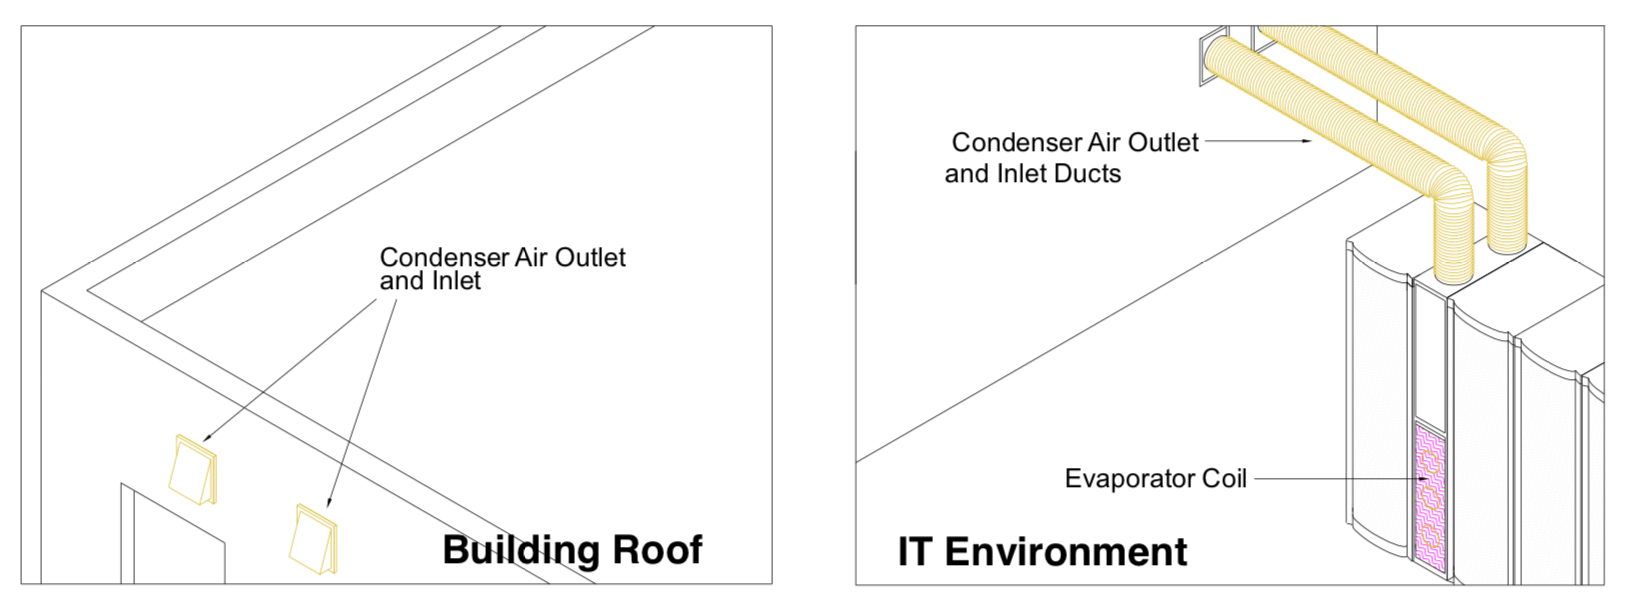
\includegraphics[width=1.0\linewidth]{crac_self_contained_schematic}
\end{frame}

\begin{frame}{Air cooled DX CRAC}
  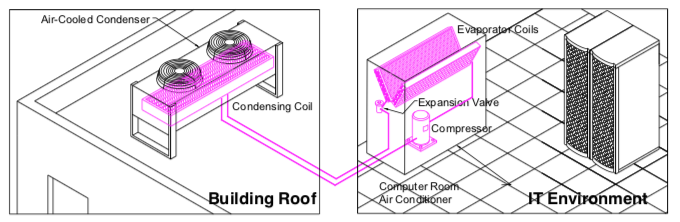
\includegraphics[width=1.0\linewidth]{crac_dx_air_schematic}
\end{frame}

\begin{frame}{Glycol-cooled DX CRAC}
  CRAC connected to dry cooler (possibly shared)\\
  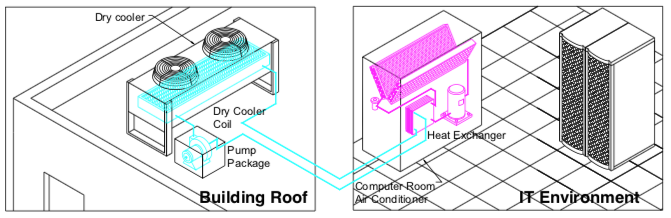
\includegraphics[width=1.0\linewidth]{crac_dx_glycol_schematic}
\end{frame}

\begin{frame}{Water-cooled DX CRAC}
  CRAC connected to cooling tower (usually shared)
  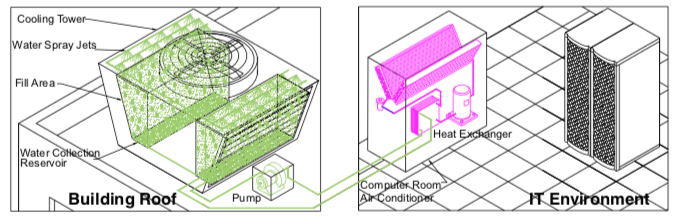
\includegraphics[width=1.0\linewidth]{crac_dx_water_schematic}
\end{frame}

\autoimage{chilled_water_system_water_cooled}

\end{document}

